\documentclass{article}




\usepackage[utf8]{inputenc}
\usepackage[T1]{fontenc}
\usepackage{amsmath} 
\usepackage{array}
\usepackage{xcolor}
\usepackage{amssymb}
\usepackage{amsthm}
\usepackage{graphicx}
\usepackage{float}


\newcommand\redu[1]{\color{red}\underline{\color{black}#1} \color{black}}
\newcommand\blueu[1]{\color{blue}\underline{\color{black}#1}\color{black}}
\newcommand\doubleu[1]{\underline{\underline{#1}}}



\author{Simon Wicky (260589) \and Jeremy Mion (261178)}
\title{Rapport Benchmarking DHT}
\date{05.2018}

\begin{document}

\maketitle
\pagenumbering{arabic}

\section{Benchmarking : Implémentation et scénarios testés}

\subsection{Implémentation}
L'implémentation de ce benchmarking en C est très brève. Elle consiste juste à chronométrer les phases réseau, c'est à dire la requête put ainsi que sa réponse, et la requête get, ainsi que sa réponse. Les différents scénario sont ensuite executés par l'intermédiaire de script bash, détaillés ci-après. \\
Les tests ont été effectués sur une liste de 40 serveurs, qui ont répondus de manière répétée et fiable à une commande pps-list-nodes

\subsection{Scénarios testés}
Les différents scénarios ont été testés :
\subsubsection{Put, couple clé-valeur fixe, N = 10, W variable}
Nous avons simulé 100 fois l'action de mettre une valeur sur la Hashtable, avec N valant 10, et W variant entre 1 et 10.\\
Le script \textbf{\textit{./test\_put}} effectue une action put, avec W partant de 1 jusqu'a 10. Le résultat est écrit dans un fichier. \\
Le script \textbf{\textit{./test\_put\_csv}} se charge de lancer 100 fois \textbf{\textit{./test\_put}}, de collecter les résultats et de les fusionner dans un seul fichier au format csv, où chaque ligne correspond à une valeur de W. \\
Les résultats récoltés sont résumés dans la Figure \ref{figPut}. \\
Il est important de noter que certains écart-types ne sont pas affichés, ceux ci étant trop élevé, suite à de probables timeout.
\begin{figure}
 	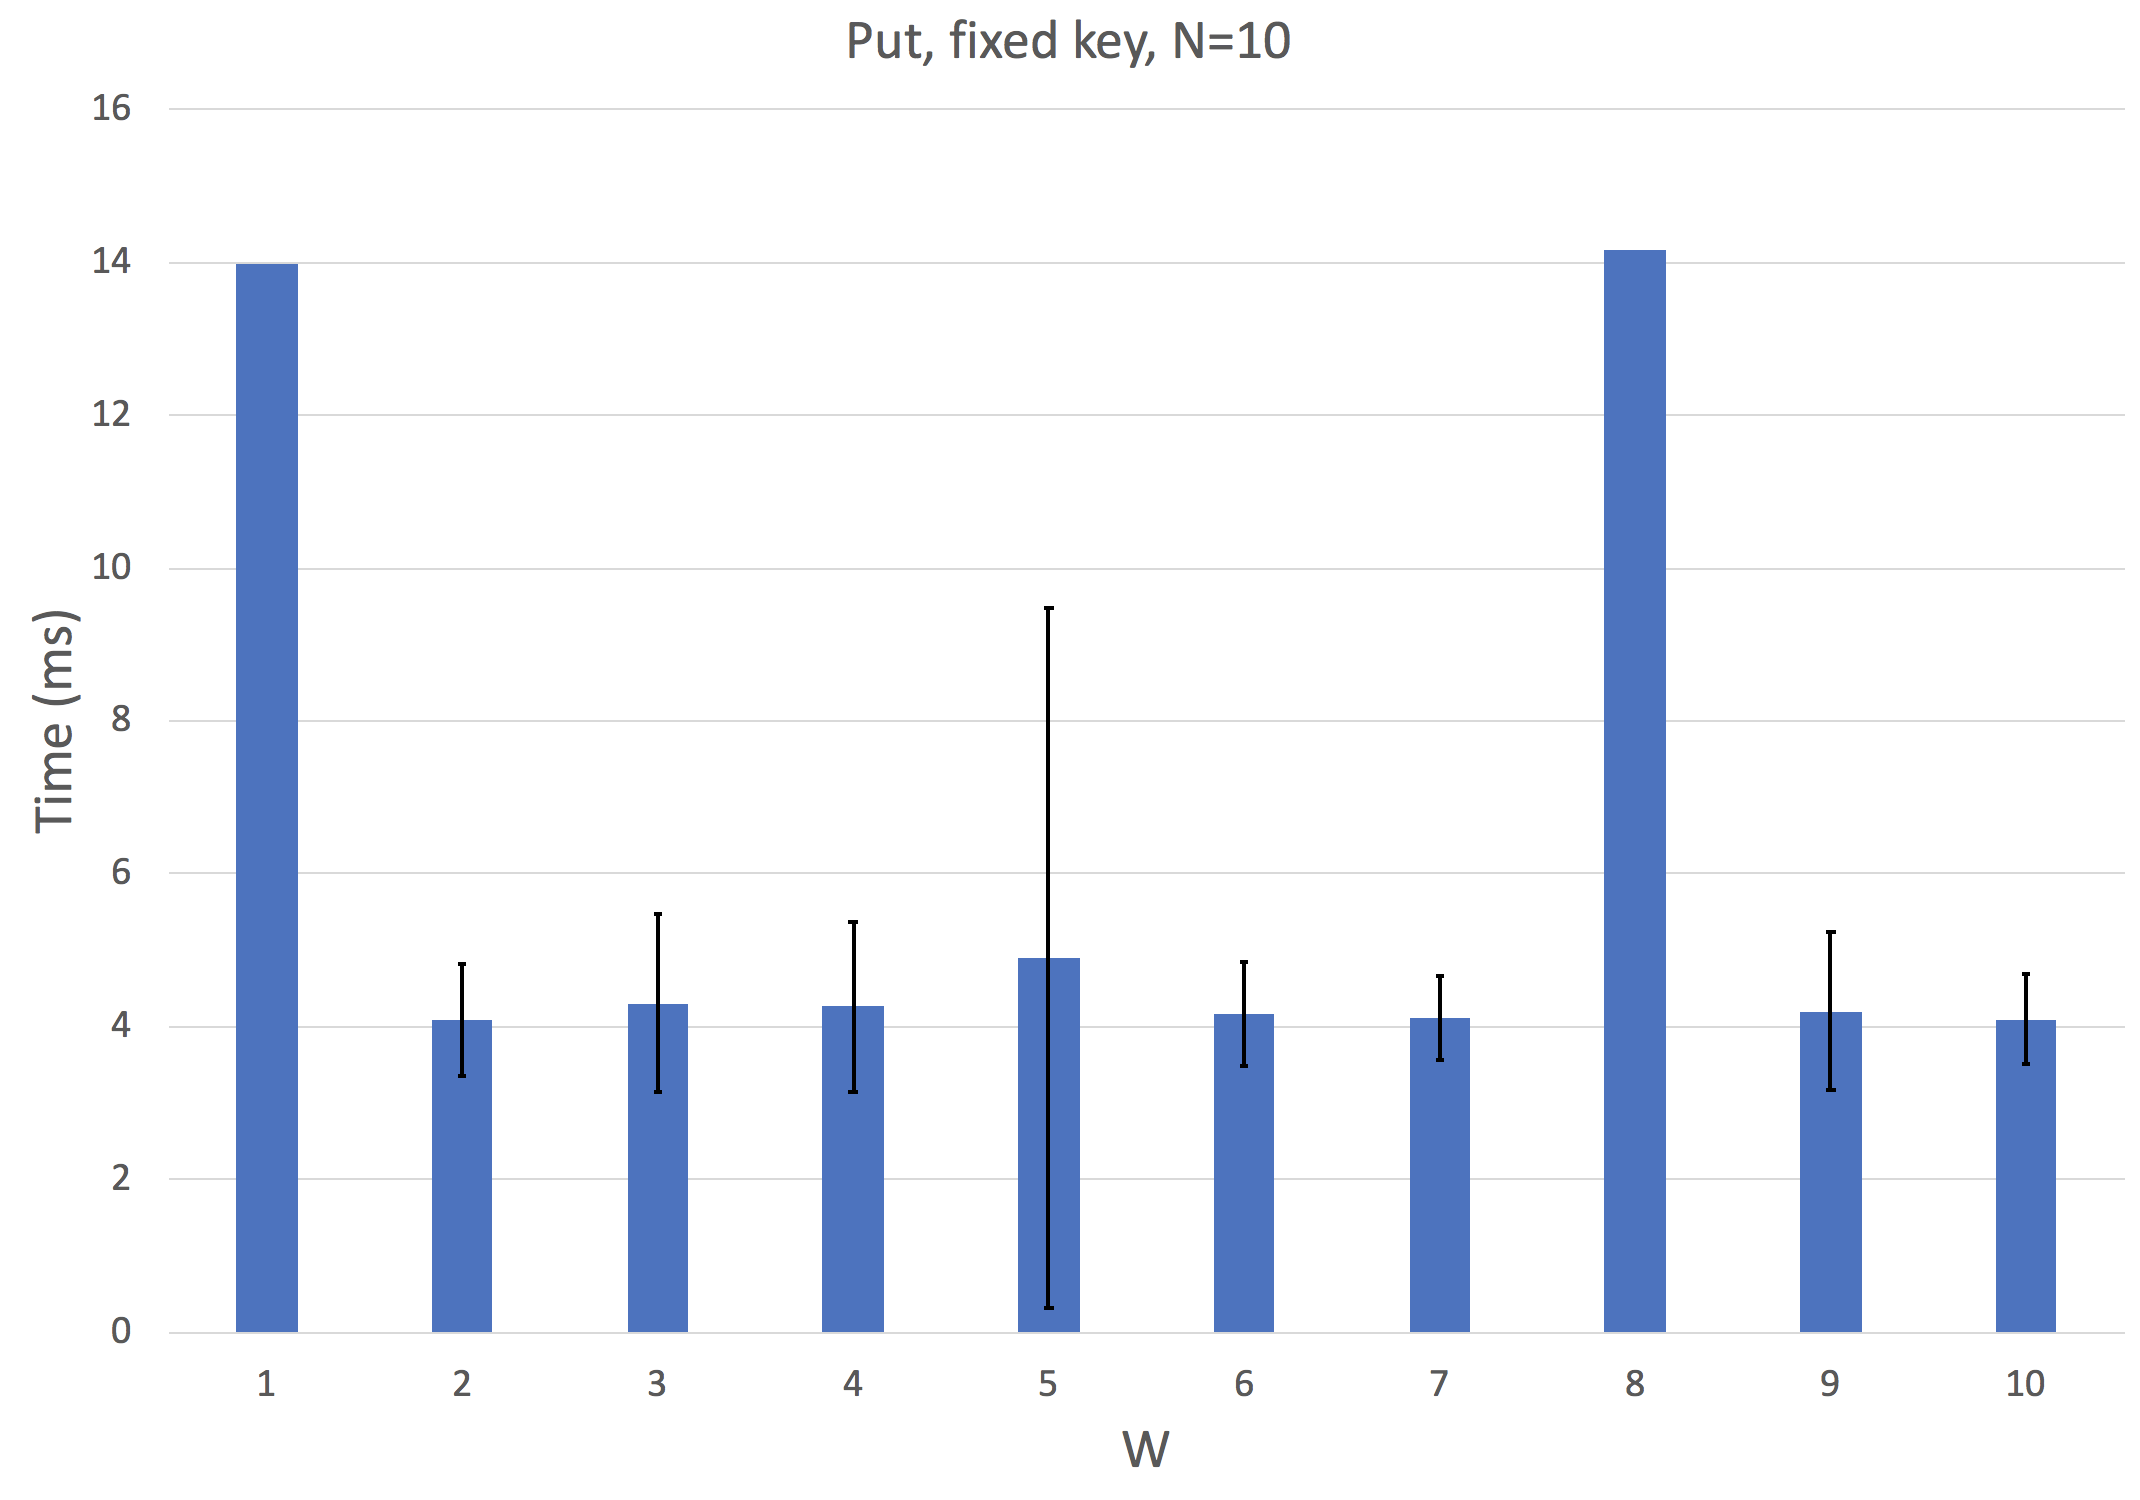
\includegraphics[scale = 0.25]{img/Put}
 	\caption{Graphique du scénario 1.2.1}
 	\label{figPut}
\end{figure}

\subsubsection{Get, couple clé-valeur fixe, N = 10, R variable}
Nous avons ensuite simulé 100 fois l'action de demander une valeur sur la Hashtable, avec N valant 10, et R variant entre 1 et 10.\\
Le script \textbf{\textit{./test\_get}} effectue une action get, avec R partant de 1 jusqu'a 10. Le résultat est écrit dans un fichier. \\
Le script \textbf{\textit{./test\_get\_csv}} se charge de lancer 100 fois \textbf{\textit{./test\_get}}, de collecter les résultats et de les fusionner dans un seul fichier au format csv, où chaque ligne correspond à une valeur de R. \\
Les résultats récoltés sont résumés dans la Figure \ref{figGet}. \\
Il est important de noter que certains écart-types ne sont pas affichés, ceux ci étant trop élevé, suite à de probables timeout.

\begin{figure}
 	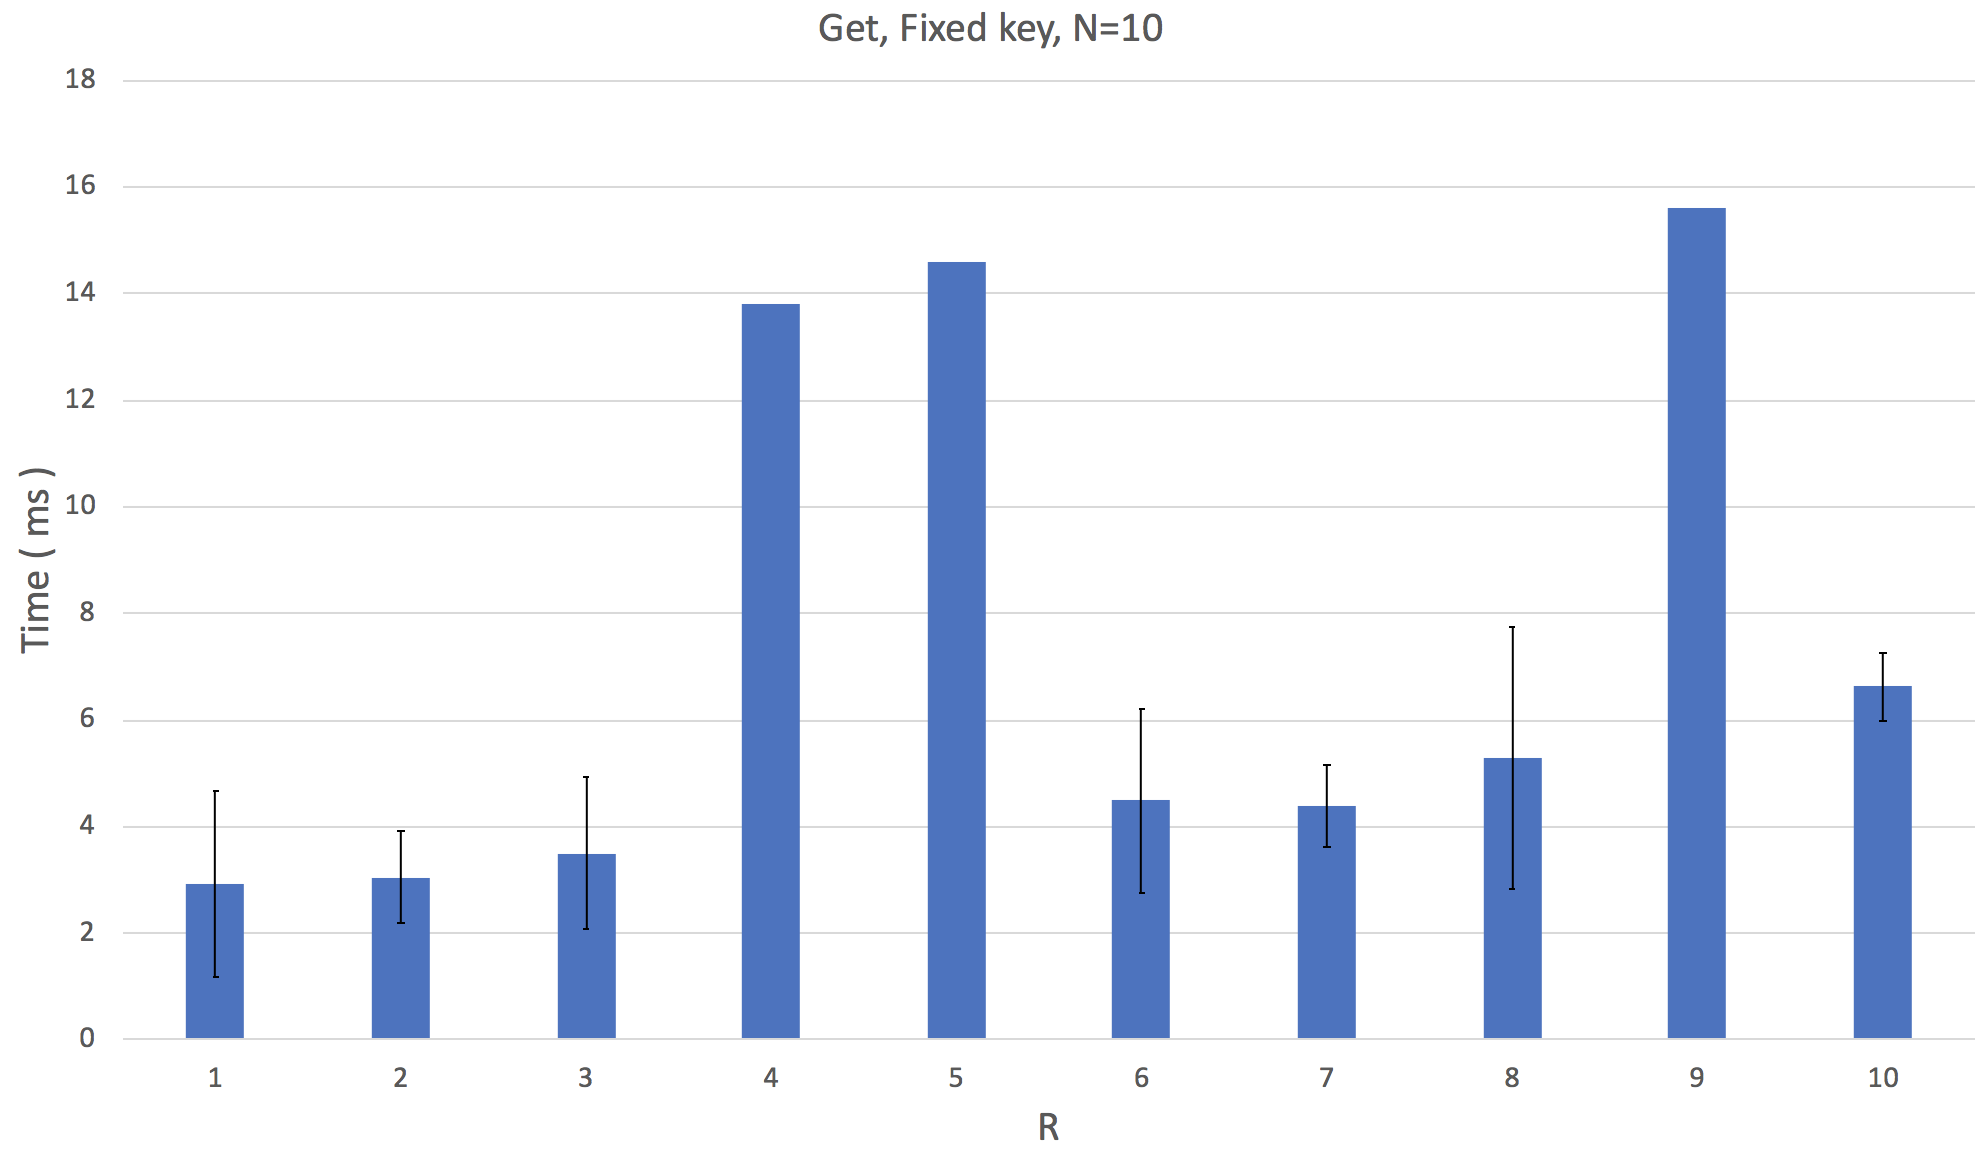
\includegraphics[scale = 0.25]{img/Get}
 	\caption{Graphique du scénario 1.2.2}
 	\label{figGet}
\end{figure}

\subsubsection{Put et Get, couple clé-valeur aléatoire}
Le dernier test consiste à mettre puis à demander un couple clé-valeur aléatoire. La taille de la clé est également aléatoire (limitée entre 1 et 1000), la taille de la valeur, elle, est fixe (100). \\
Pour ceci, les scripts \textbf{\textit{./test\_random\_key}} et \textbf{\textit{./test\_random\_key\_csv}} se charge d'effectuer 1000 opérations, et de collecter les donnés au format csv. Ces données sont représentés dans la Figure \ref{figRandom}. \\
Pour des raisons de visibilité, certaines valeurs trop élevées ont été omises.


\begin{figure}
	\center
 	\includegraphics[scale = 0.25]{img/Random.JPG}
 	\caption{Graphique du scénario 1.2.2}
 	\label{figRandom}
\end{figure}

\section{Conclusion}
Après les tests, nous remarquons que les données sont relativement variables. Cela vient en grande partie du fait que tous les serveurs sont différents, et qu'ils n'ont pas tous le comportement attendus. Certains ne gère peut etre pas certaines tailles de clés par exemple, et peuvent être la cause de plusieurs timeout. Un test plus dirigé avec des serveurs identiques exhiberait sans doute plus de résultats intéressants.







\end{document}
